\documentclass[10pt]{article}

\usepackage{fullpage}

\usepackage{tikz}

\usetikzlibrary{shapes.geometric, arrows}

\setlength{\parindent}{0pt}

\tikzstyle{boxEmulate} = [rectangle, rounded corners,  text width=4cm, minimum width=3cm, minimum height=1cm, text centered, draw=black, fill=white]

\tikzstyle{boxUtils} = [rectangle, rounded corners,  text width=6cm, minimum width=3cm, minimum height=1cm, draw=black, fill=white]

\tikzstyle{arrow} = [thick, ->, >=stealth]

\begin{document}

\title{\vspace{-2cm}ARM-11 CHECKPOINT}

\author{Top of the morning, Luqmaaaaaaan, Memory man, Hi I'm Sanchit}

\date{\today}

\maketitle

\section*{Introduction}
Our first course of action for this project was to decide which technologies we will use to manage our tasks
and keep track of our progress. After trialling a few different options, including the Microsoft Teams Planner,
we decided to use the \textsl{‘Issues’} feature within GitLab. \textsl{Issues} allowed us to keep track of both our tasks and code
progress in one place, which made the delegation and completion of tasks more streamlined. Being well coordinated was a priority in our plan for this project as it meant we could effectively carry out our tasks and successfully build up the project. We also had regular meetings, via Discord, to discuss each member’s plans
for the project, what they had completed and what they intended to complete by the end of each day. 


\section*{Task Delegation}
We collectively decided to begin creating our own implementations of the foundations for this project. This
included how the registers and memory were to be defined within our code. Upon completion of this initial
task, we had a meeting on which features from each member’s code we will use in the project. After
confirming our memory and register design, we created a list of tasks which were then split among the group.
These tasks were naturally divided into three types: \textsl{Fetch, Decode} and \textsl{Execute}.


The \textsl{'Fetch'} task was to generate several functions which handled the loading of the binary file and initialised
the state of our emulator. Morkus worked on this...
Morkus add a sentence or two here for Fetch and that memory stuff you did. 
The loading of the binary file into memory is handled by the function {\tt init\_arm}.


The \textsl{‘Decode’} task…Need to finish this


The \textsl{‘Execute’} task was split further into four types based on each of the four instructions that were to be
implemented. We decided to have one member working solely on the \textsl{Data Processing Instruction} (Alex) and another
for the \textsl{Single Data Transfer Instructions} (Sanchit) as they required more time to complete. The \textsl{Multiply} and \textsl{Branch}
instructions were relatively shorter and only needed one member to implement both functions - (Luqman).

\section*{Current Evaluation}
As a team, we feel that we have worked well together so far. Any conflicts on plans for a feature were solved
quickly, and we have not had any issues with the work ethic of any member. Our team have been using Git to
constantly commit changes with useful messages, create branches to prevent problems in the Master and
updating the Git \textsl{issues}, which all translates to a well-structured process in tackling this project.


The cohesive nature of our group is supported by the extensive internal code reviews we conduct for our
fellow members’ tasks. To ensure that we remove logical errors within our programs and improve the
definitions of some functions, we decided to work on reviewing and testing each other’s code. These code
reviews were especially helpful as minor errors are easily missed when working on code for extended periods.
Although the reviews took many hours on some occasions, each member of the group was happy to help
another. This meant that our overall implementation improved immensely. The reviews are an aspect of our
group working that we are proud of and hope to maintain throughout this project.


During the first few days, we had a small problem with the times each of us had started and ended their work
for the day, mainly due to different sleeping patterns. This staggered timing meant it was harder for us to
communicate effectively and work on the project together. However, after a constructive meeting, we solved
that problem and had every member available to work on the project or help another member within a fixed
period every day. For future implementations in this project the team has been adviced to be more open if they
are having difficulties implementing a solution to prevent wasted and time when running tests. 

\section*{Emulator Implementation}
Our aim in designing the structure of the emulator was to ensure that it was as clear as possible for an external
programmer to understand how our code worked and where everything could be found. This was achieved by
maintaining a consistent naming convention, splitting files and effectively commenting our code.


We decided to alter the initial structure of the project by incorporating additional files. This was necessary as
having all our code in one place was both difficult to work on and difficult for someone else to understand. As
a result, our {\tt emulate.c} file only consisted of the {\tt main} function which initialised the emulator. We extracted the
remainder of the code into a new file called {\tt emulate\_utils.c}. This ensured better readability and organisation in our code.
 

Another aspect of the project that we noticed had to be improved was the use of \textsl{‘magic numbers’}. We found
that our code quickly became unreadable and difficult to comprehend with several numbers used for masks
and shifts within our functions. We agreed to eliminate this issue by having clearly named pre-processor
constants at the top of our file. However, even this became too cluttered, and a better solution was needed to
uphold clarity and readability within the program. This led us to create a new header file, {\tt constants.h}, which
housed all the constants that were used in our emulator. These constants were grouped by where and how
they were used, which were indicated by comments.


The following diagram provides a brief overview of our project structure for the emulator and includes the
general contents of each file:

\vspace{0.5cm}

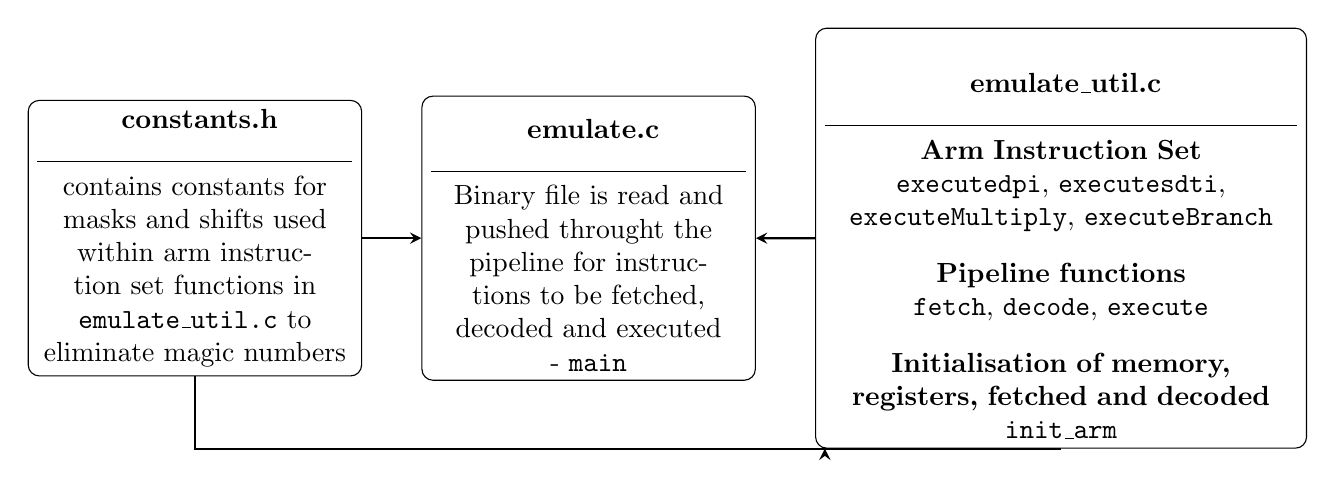
\begin{tikzpicture}[node distance=2cm]

\node (constants) [boxEmulate, yshift =10cm] {
\textbf{ constants.h} 
\rule{\textwidth}{0.4pt}
contains constants for masks and shifts used within arm instruction set functions in {\tt emulate\_util.c} to eliminate magic numbers

};

\node (emulate) [boxEmulate, right of=constants, xshift=3cm] {

\textbf{ emulate.c} 
\rule{\textwidth}{0.4pt}
Binary file is read and pushed throught the pipeline for instructions to be fetched, decoded and executed\\
 - {\tt main}

};



\node[boxUtils,xshift = 4cm, yshift = 5cm, right of=emulate] (a) at (5,5) (emulateutil){
\center\textbf{ emulate\_util.c}
\rule{\textwidth}{0.4pt}

\textbf{Arm Instruction Set} \\
{\tt executedpi},    
 {\tt executesdti}, 
 {\tt executeMultiply}, 
 {\tt executeBranch}\\
\vspace{0.3cm}
\textbf{Pipeline functions} \\
{\tt fetch},
 {\tt decode},
 {\tt execute}\\
\vspace{0.3cm}
\textbf{Initialisation of memory, registers, fetched and decoded}\\
 {\tt init\_arm}

};

\draw [arrow] (emulateutil) -- (emulate);
\draw [arrow] (constants) -- (emulate);
\draw [arrow] (constants.south) |- (emulateutil.south) + (-3,0);

\end{tikzpicture}


\section*{Upcoming Challenges}
Paragraph on which parts we will reuse:
After discussing our plans for the assembler, we found that we could [reuse these parts]
Paragraph on parts we might find difficult and how we will mitigate:
(Ways we will mitigate problems: code reviews, work together, research etc)

\end{document}
